\section{What survives execution: search extensions on a fresh cohort}
\label{sec:search}

\paragraph{Arms.}
All four arms share one code version, seed 0 and one refinement iteration. \textbf{A} is CADFit with the measurement fixes of \cref{sec:measure}. \textbf{B} adds a rule package: a persistent CadQuery interpreter (byte-identical outputs, about 90\% less per-call startup), exact-union scoring, a cut phase that subtracts candidate solids while IoU improves, event slices between consecutive heights of axis-normal planar faces, extrusion directions from clustered face normals, and a subsampled translation sweep. \textbf{C} adds beam search (width 4) over compositions. \textbf{D} adds whole-part section proposals: for each axis, the target's mid-bounding-box cross-section, simplified and extruded through the full extent of the part, enters the candidate pool. This recipe began as a control an external reviewer designed after seeing agent results on test parts; we froze it on development parts before drawing the fresh cohort. As a further control, \emph{best-of} takes, per part, whichever of C's model and the best single section extrusion has the higher IoU against the target mesh.

\begin{table}[t]
\centering
\small
\caption{Search arms on \nFresh{} fresh parts. \iouc: IoU of the solid built by executing the final program (0 if it does not build); \ioug: additionally 0 unless the shape is OpenCascade-valid. CD over parts with an output ($n$). Unbuilt + invalid: programs that do not build + built but invalid. n/m: not measured.}
\label{tab:arms}
\resizebox{\linewidth}{!}{%
\begin{tabular}{@{}lcccccccc@{}}
\toprule
 & mesh IoU & \iouc & \ioug & gap & CD ($n$) & unbuilt + inv. & \iouc{} benchA & \iouc{} benchE \\
\midrule
A base & \armBaseIou & \armBaseCad & \armBaseGated & \armBaseGap & \armBaseCd{} (\armBaseCdN) & \armBaseUnbuilt{} + \armBaseBuiltInvalid & \armBaseSplitACad & \armBaseSplitECad \\
B + rules & \armRulesIou & \armRulesCad & \armRulesGated & \armRulesGap & \armRulesCd{} (\armRulesCdN) & \armRulesUnbuilt{} + \armRulesBuiltInvalid & \armRulesSplitACad & \armRulesSplitECad \\
C + beam & \armBeamIou & \armBeamCad & \armBeamGated & \armBeamGap & \armBeamCd{} (\armBeamCdN) & \armBeamUnbuilt{} + \armBeamBuiltInvalid & \armBeamSplitACad & \armBeamSplitECad \\
D + sections & \armSecIou & \armSecCad & \armSecGated & \armSecGap & \armSecCd{} (\armSecCdN) & \armSecUnbuilt{} + \armSecBuiltInvalid & \armSecSplitACad & \armSecSplitECad \\
\midrule
best-of (C, sections) & \bestOfIou & \bestOfCad & n/m & & & n/m & & \\
sections only & \sectionsOnlyIou & & & & & & & \\
\bottomrule
\end{tabular}}

\vspace{0.6em}
\resizebox{\linewidth}{!}{%
\begin{tabular}{@{}lcccc@{}}
\toprule
paired difference & $\Delta$ mesh IoU & $\Delta$ \iouc & $\Delta$ \ioug & $\Delta$\iouc{} $-$ $\Delta$mesh \\
\midrule
B $-$ A (rules) & \dRulesBaseIouDiff{} \dRulesBaseIouCI & \dRulesBaseCadDiff{} \dRulesBaseCadCI & \dRulesBaseGatedDiff{} \dRulesBaseGatedCI & \dRulesBaseShrinkDiff{} \dRulesBaseShrinkCI \\
C $-$ B (beam) & \dBeamRulesIouDiff{} \dBeamRulesIouCI & \dBeamRulesCadDiff{} \dBeamRulesCadCI & \dBeamRulesGatedDiff{} \dBeamRulesGatedCI & \dBeamRulesShrinkDiff{} \dBeamRulesShrinkCI \\
D $-$ C (sections) & \dSecBeamIouDiff{} \dSecBeamIouCI & \dSecBeamCadDiff{} \dSecBeamCadCI & \dSecBeamGatedDiff{} \dSecBeamGatedCI & \dSecBeamShrinkDiff{} \dSecBeamShrinkCI \\
D $-$ A (all) & \dSecBaseIouDiff{} \dSecBaseIouCI & \dSecBaseCadDiff{} \dSecBaseCadCI & \dSecBaseGatedDiff{} \dSecBaseGatedCI & \dSecBaseShrinkDiff{} \dSecBaseShrinkCI \\
\bottomrule
\end{tabular}}
\end{table}

\paragraph{Mesh IoU overstates the executed program, through programs that do not build (Q1).}
The base arm's executed programs reproduce its meshes: the mean gap between mesh IoU and \iouc{} is \armBaseGap{} (\cref{tab:arms}). The gap rises to \armRulesGap{} with the rule package and \armBeamGap{} with beam search, then falls to \armSecGap{} with section proposals. In arm C, \armBeamUnbuilt{} programs do not build and \armBeamBuiltInvalid{} build but fail OpenCascade validity. Averaged over all \nFresh{} parts, the unbuilt programs contribute \armBeamGapUnbuilt{} of the \armBeamGap{} gap and built programs \armBeamGapBuilt. Built programs usually reproduce their meshes, though not always: the largest built-program discrepancy in arm C is \beamMaxBuiltGap{} (\cref{fig:scatter}).

\begin{figure}[t]
\centering
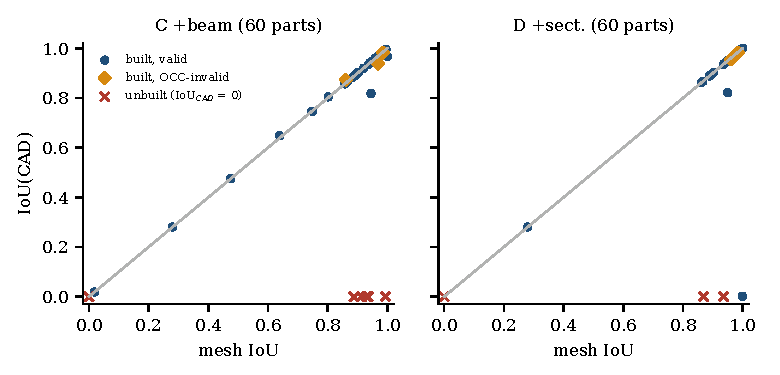
\includegraphics[width=0.62\linewidth]{figures/mesh_vs_cad.pdf}
\caption{Per-part mesh IoU against \iouc{} for arms C and D (\nFresh{} parts). Crosses: programs that do not build (plotted at 0) or build but fail OpenCascade validity. Points on the diagonal reproduce their reported mesh.}
\label{fig:scatter}
\end{figure}

\paragraph{Gains shrink when programs are executed (Q2).}
Each extension raises mean mesh IoU, and every mesh-IoU interval in \cref{tab:arms} excludes zero. The last column tests whether the executed-program gain is smaller than the mesh gain on the same parts. It is for the rule package (\dRulesBaseShrinkDiff, \dRulesBaseShrinkCI) and for the full ladder D $-$ A (\dSecBaseShrinkDiff, \dSecBaseShrinkCI); for beam search alone the test is inconclusive (\dBeamRulesShrinkCI). Win/loss counts show how a few failures dominate a mean: under \ioug, the rule package improves \dRulesBaseGatedWins{} parts and worsens \dRulesBaseGatedLosses, yet its mean change is \dRulesBaseGatedDiff, because the parts it worsens lose their whole score.

\paragraph{Whole-part section proposals survive execution, mainly on benchE (Q2).}
Section proposals are the largest observed \iouc{} increment among the extensions: D $-$ C is \dSecBeamCadDiff{} \dSecBeamCadCI, and D has the highest \iouc{} of the four arms. A single best-axis section extrusion with no search reaches a mean mesh IoU of \sectionsOnlyIou, above the base arm's \armBaseIou. Folding the proposals into the search is not distinguishable from picking the better of C and the best section per part (D $-$ best-of on \iouc: \dSecBestOfCadDiff{} \dSecBestOfCadCI). Over the base arm, the overall \iouc{} gain of D is \dSecBaseCadDiff{} \dSecBaseCadCI, and it comes from benchE (\dSecBaseSplitECadDiff{} \dSecBaseSplitECadCI) rather than benchA (\dSecBaseSplitACadDiff{} \dSecBaseSplitACadCI). The per-split estimates locate the gain without testing an interaction, and because each arm adds its rules as a package, the design separates packages, not individual rules.
